\documentclass[tikz,border=8pt]{standalone}
\usepackage[T1]{fontenc}
\usepackage{amsmath,amssymb}
\usepackage{xcolor}
\usepackage{tikz}
% Shared TikZ style for the DEV architecture diagrams.
% Requires only TikZ and standard TikZ libraries.
\usetikzlibrary{arrows.meta,backgrounds,calc,fit,positioning}

\definecolor{DevInk}{HTML}{172033}
\definecolor{DevMuted}{HTML}{526078}
\definecolor{DevLine}{HTML}{475569}
\definecolor{DevPanel}{HTML}{F8FAFC}
\definecolor{DevPanelBorder}{HTML}{CBD5E1}
\definecolor{DevContent}{HTML}{DBEAFE}
\definecolor{DevContentBorder}{HTML}{2563EB}
\definecolor{DevStyle}{HTML}{F3E8FF}
\definecolor{DevStyleBorder}{HTML}{9333EA}
\definecolor{DevStable}{HTML}{DCFCE7}
\definecolor{DevStableBorder}{HTML}{16A34A}
\definecolor{DevAllograph}{HTML}{FFEDD5}
\definecolor{DevAllographBorder}{HTML}{EA580C}
\definecolor{DevCritic}{HTML}{FEE2E2}
\definecolor{DevCriticBorder}{HTML}{DC2626}
\definecolor{DevLoss}{HTML}{FEF3C7}
\definecolor{DevLossBorder}{HTML}{D97706}

\tikzset{
  devtext/.style={font=\sffamily\small, text=DevInk, align=center},
  devbox/.style={
    devtext,
    draw=DevPanelBorder,
    fill=white,
    rounded corners=2.2mm,
    line width=0.75pt,
    inner xsep=3.2mm,
    inner ysep=2.4mm,
    minimum height=9mm
  },
  devinput/.style={devbox, draw=DevContentBorder, fill=DevContent},
  devcontent/.style={devbox, draw=DevContentBorder, fill=DevContent},
  devstyle/.style={devbox, draw=DevStyleBorder, fill=DevStyle},
  devstable/.style={devbox, draw=DevStableBorder, fill=DevStable},
  devallograph/.style={devbox, draw=DevAllographBorder, fill=DevAllograph},
  devcritic/.style={devbox, draw=DevCriticBorder, fill=DevCritic},
  devloss/.style={devbox, draw=DevLossBorder, fill=DevLoss},
  devgroup/.style={
    draw=DevPanelBorder,
    fill=DevPanel,
    rounded corners=3mm,
    line width=0.75pt,
    inner sep=4mm
  },
  devflow/.style={
    -{Latex[length=2.8mm,width=1.9mm]},
    draw=DevLine,
    line width=0.85pt,
    rounded corners=1.4mm
  },
  devaux/.style={
    devflow,
    draw=DevStableBorder,
    densely dashed
  },
  devlossflow/.style={
    devflow,
    draw=DevLossBorder,
    densely dashed
  },
  devlabel/.style={
    font=\sffamily\scriptsize,
    text=DevMuted,
    fill=white,
    inner sep=1.2pt
  },
  devgrouptitle/.style={
    font=\sffamily\bfseries\small,
    text=DevInk,
    fill=DevPanel,
    inner xsep=2mm,
    inner ysep=0.6mm
  },
  devnote/.style={
    font=\sffamily\scriptsize,
    text=DevMuted,
    align=left
  }
}



\begin{document}
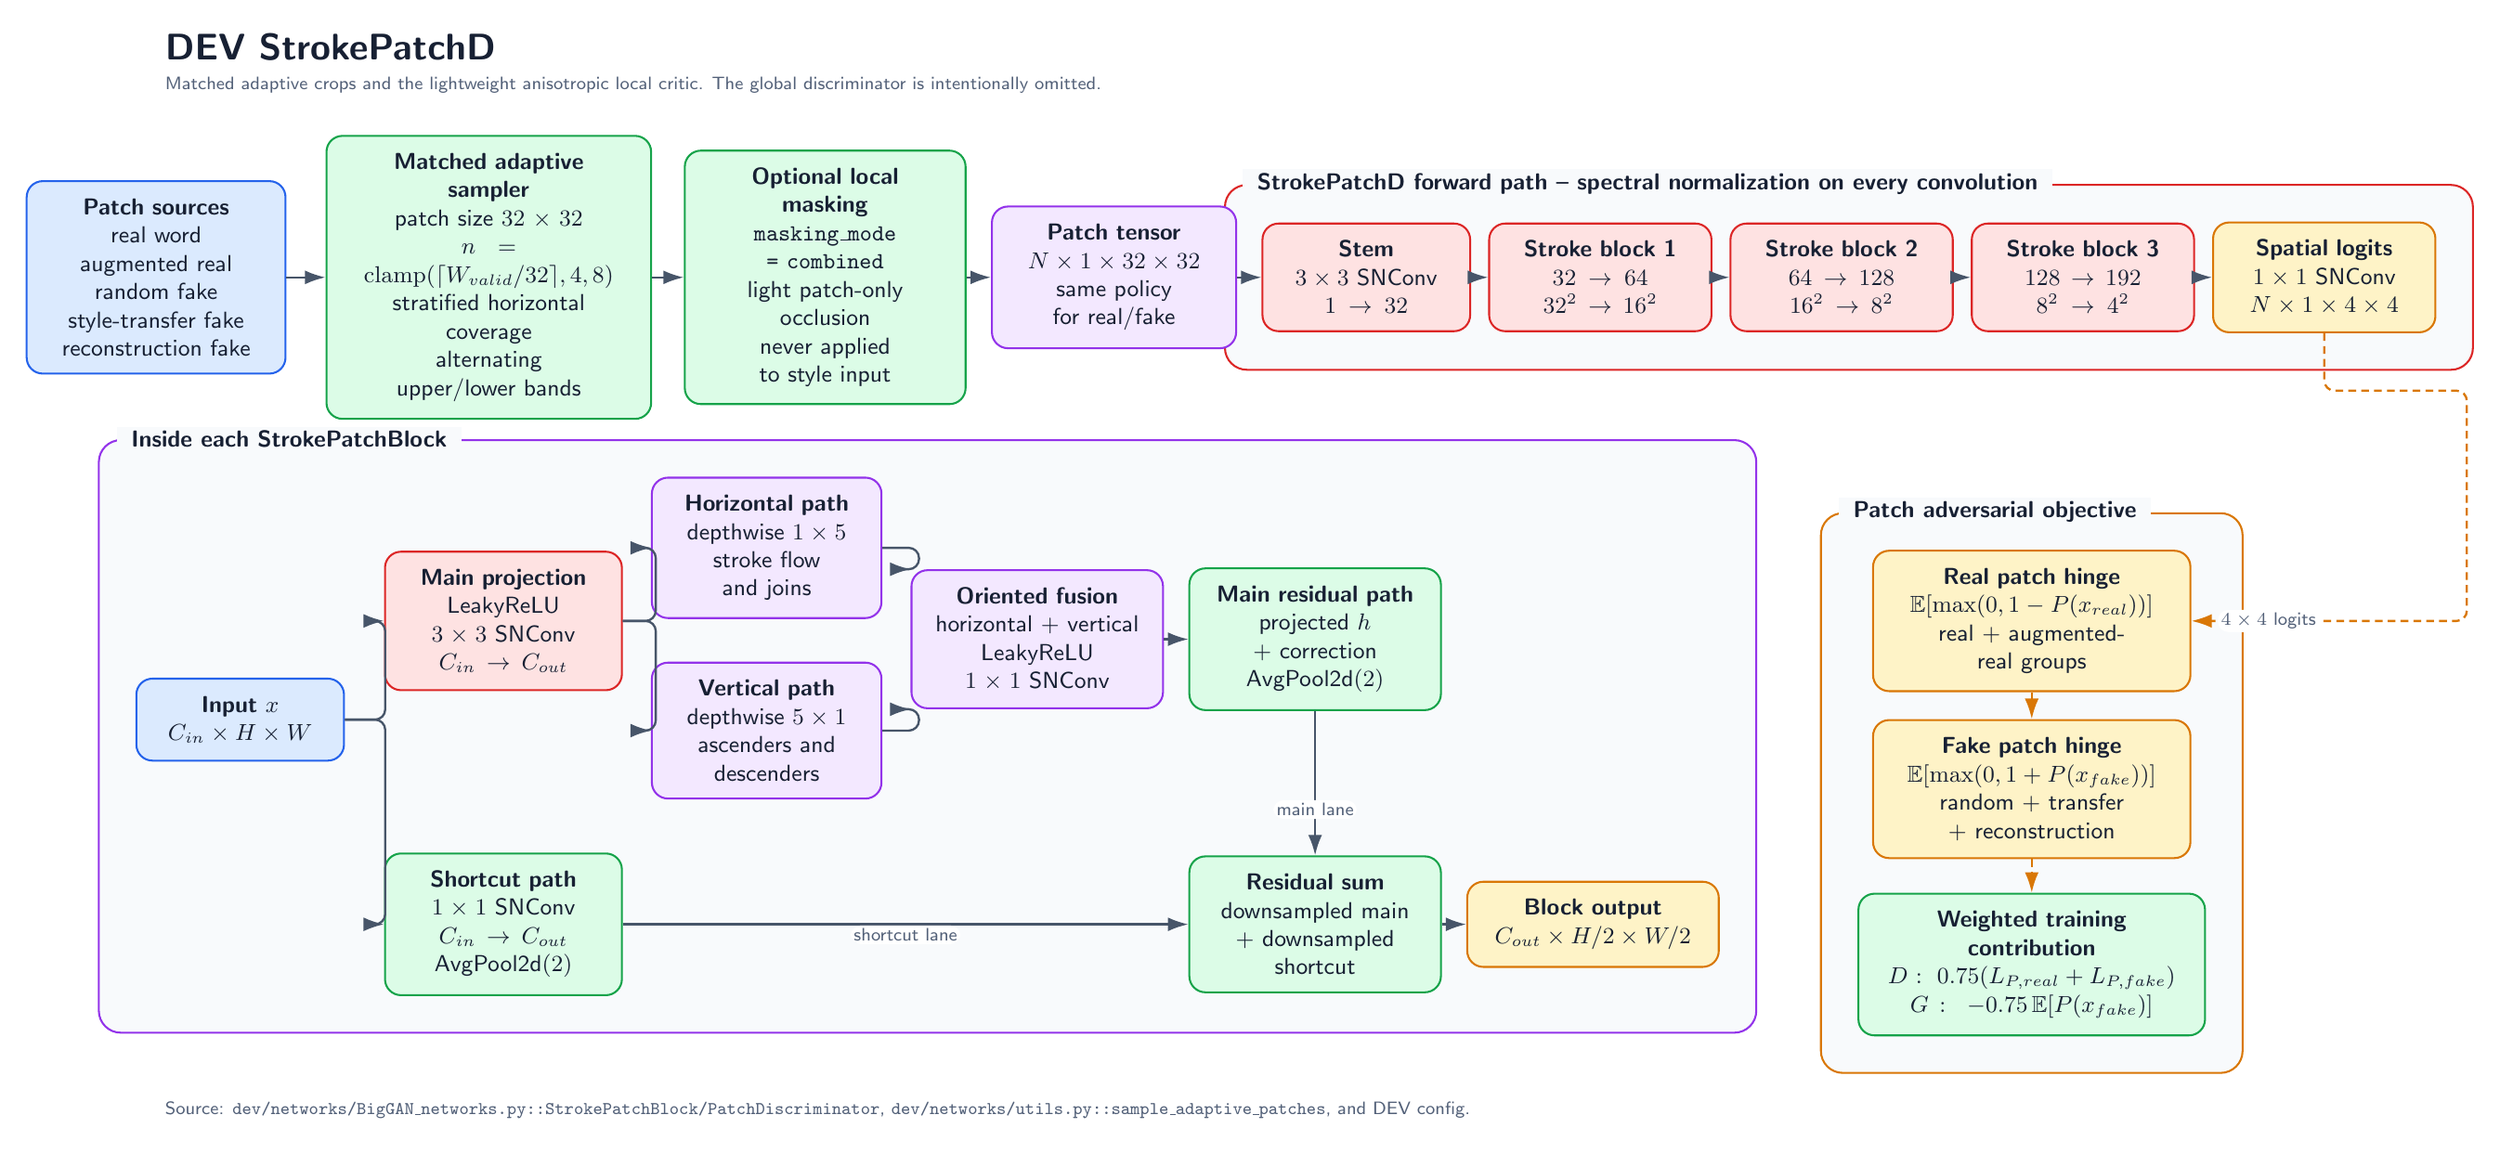
\begin{tikzpicture}[x=1cm,y=1cm]
  \node[font=\sffamily\bfseries\Large, text=DevInk, anchor=west]
    at (0,12.8) {DEV StrokePatchD};
  \node[devnote, anchor=west]
    at (0,12.28) {Matched adaptive crops and the lightweight anisotropic local critic. The global discriminator is intentionally omitted.};

  % Patch preparation path.
  \node[devinput, text width=2.9cm] (sources) at (0,9.65)
    {\textbf{Patch sources}\\real word\\augmented real\\random fake\\style-transfer fake\\reconstruction fake};
  \node[devstable, text width=3.8cm] (sampler) at (4.55,9.65)
    {\textbf{\mbox{Matched adaptive} sampler}\\patch size $32\times32$\\$n=\mathrm{clamp}(\lceil W_{valid}/32\rceil,4,8)$\\\mbox{stratified horizontal} coverage\\alternating \mbox{upper/lower} bands};
  \node[devstable, text width=3.2cm] (patchmask) at (9.15,9.65)
    {\textbf{\mbox{Optional local} masking}\\\texttt{masking\_mode}\\\texttt{= combined}\\light \mbox{patch-only} occlusion\\never applied to style input};
  \node[devstyle, text width=2.7cm] (patches) at (13.1,9.65)
    {\textbf{Patch tensor}\\$N\times1\times32\times32$\\same policy for real/fake};

  \draw[devflow] (sources) -- (sampler);
  \draw[devflow] (sampler) -- (patchmask);
  \draw[devflow] (patchmask) -- (patches);

  % PatchDiscriminator forward pipeline.
  \node[devcritic, text width=2.2cm] (stem) at (16.55,9.65)
    {\textbf{Stem}\\$3\times3$ SNConv\\$1\rightarrow32$};
  \node[devcritic, text width=2.4cm] (blockone) at (19.75,9.65)
    {\textbf{Stroke block 1}\\$32\rightarrow64$\\$32^2\rightarrow16^2$};
  \node[devcritic, text width=2.4cm] (blocktwo) at (23.05,9.65)
    {\textbf{Stroke block 2}\\$64\rightarrow128$\\$16^2\rightarrow8^2$};
  \node[devcritic, text width=2.4cm] (blockthree) at (26.35,9.65)
    {\textbf{Stroke block 3}\\$128\rightarrow192$\\$8^2\rightarrow4^2$};
  \node[devloss, text width=2.4cm] (logits) at (29.65,9.65)
    {\textbf{Spatial logits}\\$1\times1$ SNConv\\$N\times1\times4\times4$};

  \draw[devflow] (patches) -- (stem);
  \draw[devflow] (stem) -- (blockone);
  \draw[devflow] (blockone) -- (blocktwo);
  \draw[devflow] (blocktwo) -- (blockthree);
  \draw[devflow] (blockthree) -- (logits);

  % Detailed StrokePatchBlock internals. Main and shortcut paths use different
  % vertical lanes and merge only at the residual sum.
  \node[devcontent, text width=2.2cm] (blockinput) at (1.15,3.6)
    {\textbf{Input $x$}\\$C_{in}\times H\times W$};
  \node[devcritic, text width=2.6cm] (mainproj) at (4.75,4.95)
    {\textbf{Main projection}\\LeakyReLU\\$3\times3$ SNConv\\$C_{in}\rightarrow C_{out}$};
  \node[devstyle, text width=2.5cm] (horizontal) at (8.35,5.95)
    {\textbf{Horizontal path}\\depthwise $1\times5$\\stroke flow and joins};
  \node[devstyle, text width=2.5cm] (vertical) at (8.35,3.45)
    {\textbf{Vertical path}\\depthwise $5\times1$\\ascenders and\\descenders};
  \node[devstyle, text width=2.8cm] (oriented) at (12.05,4.70)
    {\textbf{Oriented fusion}\\horizontal $+$ vertical\\LeakyReLU\\$1\times1$ SNConv};
  \node[devstable, text width=2.8cm] (mainres) at (15.85,4.70)
    {\textbf{Main residual path}\\projected $h$ + correction\\AvgPool2d$(2)$};

  \node[devstable, text width=2.6cm] (shortcut) at (4.75,0.80)
    {\textbf{Shortcut path}\\$1\times1$ SNConv\\$C_{in}\rightarrow C_{out}$\\AvgPool2d$(2)$};
  \node[devstable, text width=2.8cm] (residualsum) at (15.85,0.80)
    {\textbf{Residual sum}\\\mbox{downsampled} main\\$+$ \mbox{downsampled} shortcut};
  \node[devloss, text width=2.8cm] (blockoutput) at (19.65,0.80)
    {\textbf{Block output}\\$C_{out}\times H/2\times W/2$};

  \draw[devflow] (blockinput.east) -- ++(0.55,0) |- (mainproj.west);
  \draw[devflow] (blockinput.east) -- ++(0.55,0) |- (shortcut.west);
  \draw[devflow] (mainproj.east) -- ++(0.45,0) |- (horizontal.west);
  \draw[devflow] (mainproj.east) -- ++(0.45,0) |- (vertical.west);
  \draw[devflow] (horizontal.east) -- ++(0.5,0) |- (oriented.north west);
  \draw[devflow] (vertical.east) -- ++(0.5,0) |- (oriented.south west);
  \draw[devflow] (oriented) -- (mainres);
  \draw[devflow] (mainres.south) -- ++(0,-0.55) -| node[devlabel,pos=0.78] {main lane} (residualsum.north);
  \draw[devflow] (shortcut) -- node[devlabel,below] {shortcut lane} (residualsum);
  \draw[devflow] (residualsum) -- (blockoutput);

  \begin{scope}[on background layer]
    \node[devgroup, draw=DevCriticBorder,
      fit=(stem)(blockone)(blocktwo)(blockthree)(logits), inner sep=5mm] (forwardgroup) {};
    \node[devgroup, draw=DevStyleBorder,
      fit=(blockinput)(mainproj)(horizontal)(vertical)(oriented)(mainres)(shortcut)(residualsum)(blockoutput), inner sep=5mm] (blockgroup) {};
  \end{scope}
  \node[devgrouptitle, anchor=west] at ($(forwardgroup.north west)+(0.25,0)$)
    {StrokePatchD forward path -- spectral normalization on every convolution};
  \node[devgrouptitle, anchor=west] at ($(blockgroup.north west)+(0.25,0)$)
    {Inside each StrokePatchBlock};

  % Patch-only objective. The logit route stays on the far-right margin and
  % enters the loss group from above, so it never crosses the block internals.
  \node[devloss, text width=3.7cm] (realhinge) at (25.65,4.95)
    {\textbf{Real patch hinge}\\$\mathbb{E}[\max(0,1-P(x_{real}))]$\\real + augmented-real groups};
  \node[devloss, text width=3.7cm] (fakehinge) at (25.65,2.65)
    {\textbf{Fake patch hinge}\\$\mathbb{E}[\max(0,1+P(x_{fake}))]$\\random + transfer + reconstruction};
  \node[devstable, text width=4.1cm] (weightedloss) at (25.65,0.25)
    {\textbf{\mbox{Weighted training} contribution}\\$D:\;0.75(L_{P,real}+L_{P,fake})$\\$G:\;-0.75\,\mathbb{E}[P(x_{fake})]$};

  \coordinate (logitlane) at (31.6,8.1);
  \draw[devlossflow] (logits.south) -- (29.65,8.1) -- (logitlane) |- node[devlabel,pos=0.86] {$4\times4$ logits} (realhinge.east);
  \draw[devlossflow] (realhinge) -- (fakehinge);
  \draw[devlossflow] (fakehinge) -- (weightedloss);

  \begin{scope}[on background layer]
    \node[devgroup, draw=DevLossBorder,
      fit=(realhinge)(fakehinge)(weightedloss), inner sep=5mm] (lossgroup) {};
  \end{scope}
  \node[devgrouptitle, anchor=west] at ($(lossgroup.north west)+(0.25,0)$)
    {Patch adversarial objective};

  \node[devnote, anchor=west] at (0,-1.75)
    {Source: \texttt{dev/networks/BigGAN\_networks.py::StrokePatchBlock/PatchDiscriminator}, \texttt{dev/networks/utils.py::sample\_adaptive\_patches}, and DEV config.};
\end{tikzpicture}
\end{document}

